% !TEX encoding = UTF-8 Unicode
\documentclass[../天体物理基础.tex]{subfiles}
\usepackage{xr}
\externaldocument{../天体物理基础}

\begin{document}
\section{恒星、致密星和行星}
\subsection{恒星的结构}
本节中我们将会建立简单的恒星模型。在球对称的前提下,给定恒星的初始质量,化学组成和边界条件,在某一特定半径的球壳处求解一些方程便可大致确定恒星的性质。这些方程包括质量连续性方程、流体静力学平衡方程、能量守恒方程、能量传输方程、物态方程、产能率公式和不透明度公式。我们会在各个小节的叙述中慢慢了解恒星的一些性质并补完这些方程。其中质量连续性方程
\begin{equation}
\mathrm{d}M_{r}=4\pi r^{2}\rho\left(r\right)\mathrm{d}r
\end{equation}
和流体静力学方程
\begin{equation}
\frac{\mathrm{d}P}{\mathrm{d}r}=-\frac{GM_{r}\rho\left(r\right)}{r^{2}}\label{2.1.2}
\end{equation}
比较显然就不赘述了。

\subsubsection{恒星的能量来源}
太阳为我们的地球提供了大量的光和热,一个很自然的问题便出现在科学家的脑海中:恒星的能量来源是什么?有人认为来自氢氧合成水过程中所释放的化学能 (Herschel, 1837),有人认为来自小行星撞击恒星所提供的能量 (Mayer, 1846). 一个看起来比较靠谱的猜想是引力能的释放 (Waterson, Helmholtz, Kelvin, 1850). 恒星不断向外辐射能量,内能降低导致压力下降,此时为了平衡引力恒星就会收缩,引力能再次过程中转化为内能。那么这个过程足以维持数亿年的辐射吗?简单计算恒星的引力能为
\begin{align}
\mathrm{d}U_{\text{g},i}&=-G\frac{M_{r}\mathrm{d}m_{i}}{r},\notag\\
U_{\text{g}}&=-G\int_{0}^{R}\frac{4}{3}\pi r^{3}\rho \frac{4\pi r^{2}\rho\mathrm{d}r}{r}\notag\\
&=-G\int_{0}^{R}\frac{16}{3}\pi^{2}r^{4}\rho^{2}\mathrm{d}r=-\frac{16}{15}\pi^{2}G\rho^{2}R^{5}=-\frac{3}{5}\frac{GM^{2}}{R}.
\end{align}
以太阳为例,假设引力能全部转换为辐射能,所维持的时间也不过
\begin{equation}
\tau\sim\frac{GM_{\odot}^{2}}{R_{\odot}L_{\odot}}\sim10^{7}\,\mathrm{yr}.
\end{equation}
因此人们还需寻找其他类型的能源。

到了 1920 年代,卢瑟福等人已经测定了原子核的质量,同时相对论质能方程的提出让人们意识到恒星的能量可能来自于热核反应。那么,恒星内部的环境满足进行核聚变的条件吗?我们先估计一下电荷数最小的氢原子聚变所需克服的经典库仑势垒。取质子直径$r\sim10^{-13}\,\mathrm{cm}$,所需的温度为
\begin{align}
\frac{1}{2}m_{\mathrm{H}}v^{2}&=\frac{3}{2}k_{\text{B}}T_{\text{classical}}=\frac{1}{4\pi\varepsilon_{0}}\frac{Z_{1}Z_{2}e^{2}}{r},\\
T_{\text{classical}}&=\frac{Z_{1}Z_{2}e^{2}}{6\pi\varepsilon_{0}k_{\text{B}}r}\sim10^{10}\,\mathrm{K}.
\end{align}
对于恒星来讲这个温度实在是难以达到。好在量子图景下,即使核子动能不足以跨越库仑势垒,它也有一定的概率穿越它。我们可以估算一下此时所需的温度:
\begin{align}
\frac{1}{4\pi\varepsilon_{0}}\frac{Z_{1}Z_{2}e^{2}}{\lambda}&=\frac{p^{2}}{2m_{\mathrm{H}}}=\frac{\left(h/\lambda\right)^{2}}{2m_{\mathrm{H}}},\\
\lambda&=\frac{2\pi\varepsilon_{0}h^{2}}{Z_{1}Z_{2}e^{2}m_{\mathrm{H}}}\to r,\\
T_{\text{quantum}}&=\frac{Z_{1}^{2}Z_{2}^{2}e^{4}m_{\mathrm{H}}}{12\pi^{2}\varepsilon_{0}^{2}k_{\text{B}}h^{2}}\sim10^{7}\,\mathrm{K}.
\end{align}
这个温度就比较容易达到了。我们可以来估计一下太阳内部的压力和温度。根据 (\ref{2.1.2}) 式可知,
\begin{equation}
P=\int_{0}^{P}\mathrm{d}P=\int_{R}^{0}-\frac{GM_{r}\rho}{r^{2}}\mathrm{d}r=\int_{R}^{0}-\frac{G4\pi{}r^{3}\rho^{2}}{3r^{2}}\mathrm{d}r=\frac{2\pi{}}{3}\rho^{2}GR^{2},\overline{P}\sim10^{14}\,\mathrm{Pa},
\end{equation}
因此太阳平均温度可达$T=\dfrac{\mu m_{\mathrm{H}}\overline{P}}{k_{\text{B}}\rho}\sim5\times10^{6}\,\mathrm{K}$,核心温度可达$1.5\times10^{7}\,\mathrm{K}$,足以进行氢的热核反应。

热核反应的速率取决于粒子速度分布和反应截面(沿用了散射截面的概念,表征具有某速度粒子穿越库仑势垒的概率)。粒子速度越高反应截面越大,但由于粒子分布大多满足麦克斯韦速度分布,因此速度越高粒子数越少,因此速度在一定区间内的粒子才能进行有效的反应,这个区间也被称作 Gamov 窗口。

氢核聚变是最为常见的热核反应,其核反应方程式为
\begin{equation}
4{}^{1}\mathrm{H}\to{}^{4}\mathrm{He}+2\mathrm{e}^{+}+2\nu_{\mathrm{e}}+\text{energy}.
\end{equation}
此过程中释放的能量为$E=\left(4m_{\mathrm{H}}-m_{\mathrm{He}}\right)c^{2}=4\times10^{-5}\,\mathrm{erg}$,燃烧效率$0.7\%$.

氢燃烧的方式有两种,一是质子{}-{}质子链 (proton-proton chain, pp chain),二是碳氮氧循环。pp chain 的速率$\propto T^{4}$, CNO 循环的速率$\propto{}T^{20}$,温度高于$1.5\times10^{7}\,\mathrm{K}$时 CNO 效率更高。因此前者主要发生在质量$M<1.1\,M_{\odot}$的恒星中,后者发生在$M>1.1\,M_{\odot}$的恒星中。

质子{}-{}链又可分为三种路径,记作 pp\uppercase\expandafter{\romannumeral1}, pp\uppercase\expandafter{\romannumeral2}, pp\uppercase\expandafter{\romannumeral3},其中 pp\uppercase\expandafter{\romannumeral1}最重要。
\begin{figure}[!htbp]
\centering
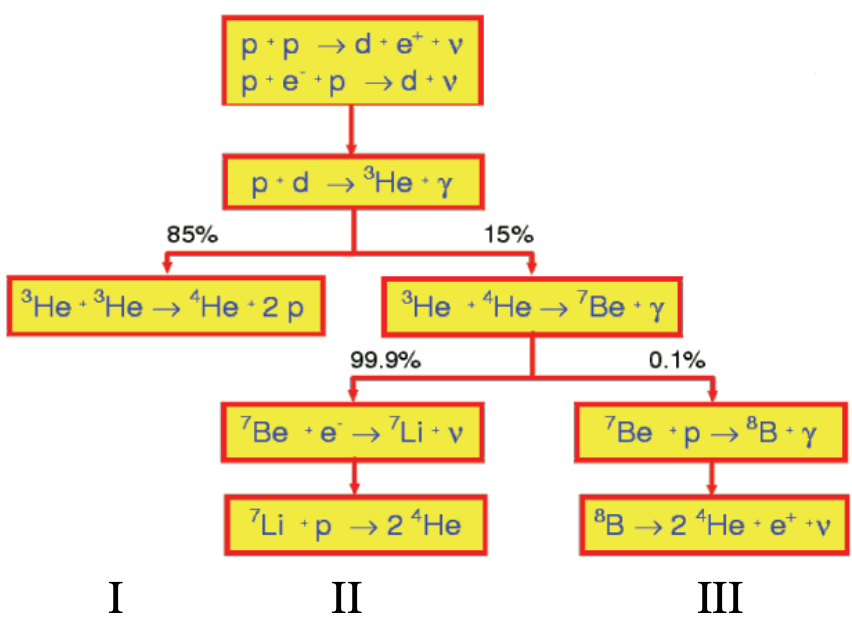
\includegraphics[width=11cm]{figures/figure2_1.png}
\captionsetup{justification=raggedright, singlelinecheck=false}
\caption{质子{}-{}质子链示意图。}
\label{ppchain}
\end{figure}

碳氮氧循环的路径则为
\begin{align*}
{}^{12}\mathrm{C}+{}^{1}\mathrm{H}&\to{}^{13}\mathrm{N}+\gamma,\\
{}^{13}\mathrm{N}&\to{}^{13}\mathrm{C}+\mathrm{e}^{+}+\nu_{\mathrm{e}},\\
{}^{13}\mathrm{C}+{}^{1}\mathrm{H}&\to{}^{14}\mathrm{N}+\gamma,\\
{}^{14}\mathrm{N}+{}^{1}\mathrm{H}&\to{}^{15}\mathrm{O}+\gamma,\\
{}^{15}\mathrm{O}&\to{}^{15}\mathrm{N}+\mathrm{e}^{+}+\nu_{\mathrm{e}},\\
{}^{15}\mathrm{N}+{}^{1}\mathrm{H}&\to{}^{12}\mathrm{C}+{}^{4}\mathrm{He}.
\end{align*}

温度高于$10^{8}\,\mathrm{K}$,将会进行氦燃烧:
\begin{align*}
{}^{4}\mathrm{He}+{}^{4}\mathrm{He}&\to{}^{8}\mathrm{Be},\\
{}^{8}\mathrm{Be}+{}^{4}\mathrm{He}&\to{}^{12}\mathrm{C}+\gamma.
\end{align*}

温度高于$5\times10^{8}\,\mathrm{K}$时进行碳燃烧,共有五种路径:
\begin{align}
{}^{12}\mathrm{C}+{}^{12}\mathrm{C}&\to{}^{24}\mathrm{Mg}+\gamma,\notag\\
&\to{}^{23}\mathrm{Na}+\mathrm{p},\notag\\
&\to{}^{20}\mathrm{Ne}+{}^{4}\mathrm{He},\notag\\
&\to{}^{23}\mathrm{Mg}+\mathrm{n},\notag\\
&\to{}^{16}\mathrm{O}+2{}^{4}\mathrm{He}.\notag
\end{align}

温度高于$1.5\times10^{9}\,\mathrm{K}$时进行氧燃烧
\begin{align}
{}^{16}\mathrm{O}+{}^{16}\mathrm{O}&\to{}^{32}\mathrm{S}+\gamma,\notag\\
&\to{}^{31}\mathrm{P}+\mathrm{p},\notag\\
&\to{}^{28}\mathrm{Si}+{}^{4}\mathrm{He},\notag\\
&\to{}^{31}\mathrm{S}+\mathrm{n},\notag\\
&\to{}^{24}\mathrm{Mg}+2{}^{4}\mathrm{He}.\notag
\end{align}

温度高于$3\times10^{9}\,\mathrm{K}$时进行硅燃烧
\begin{align}
{}^{28}\mathrm{Si}+{}^{28}\mathrm{Si}&\to{}^{56}\mathrm{Ni}+\gamma,\notag\\
{}^{56}\mathrm{Ni}&\to{}^{56}\mathrm{Fe}+2\mathrm{e}^{+}+2\nu_{\mathrm{e}}.\notag
\end{align}

更重元素的燃烧要求核心有更高的温度。热核反应导致恒星内部形成洋葱状结构,越里面的元素越重,温度越高。
\begin{figure}[!htbp]
\centering
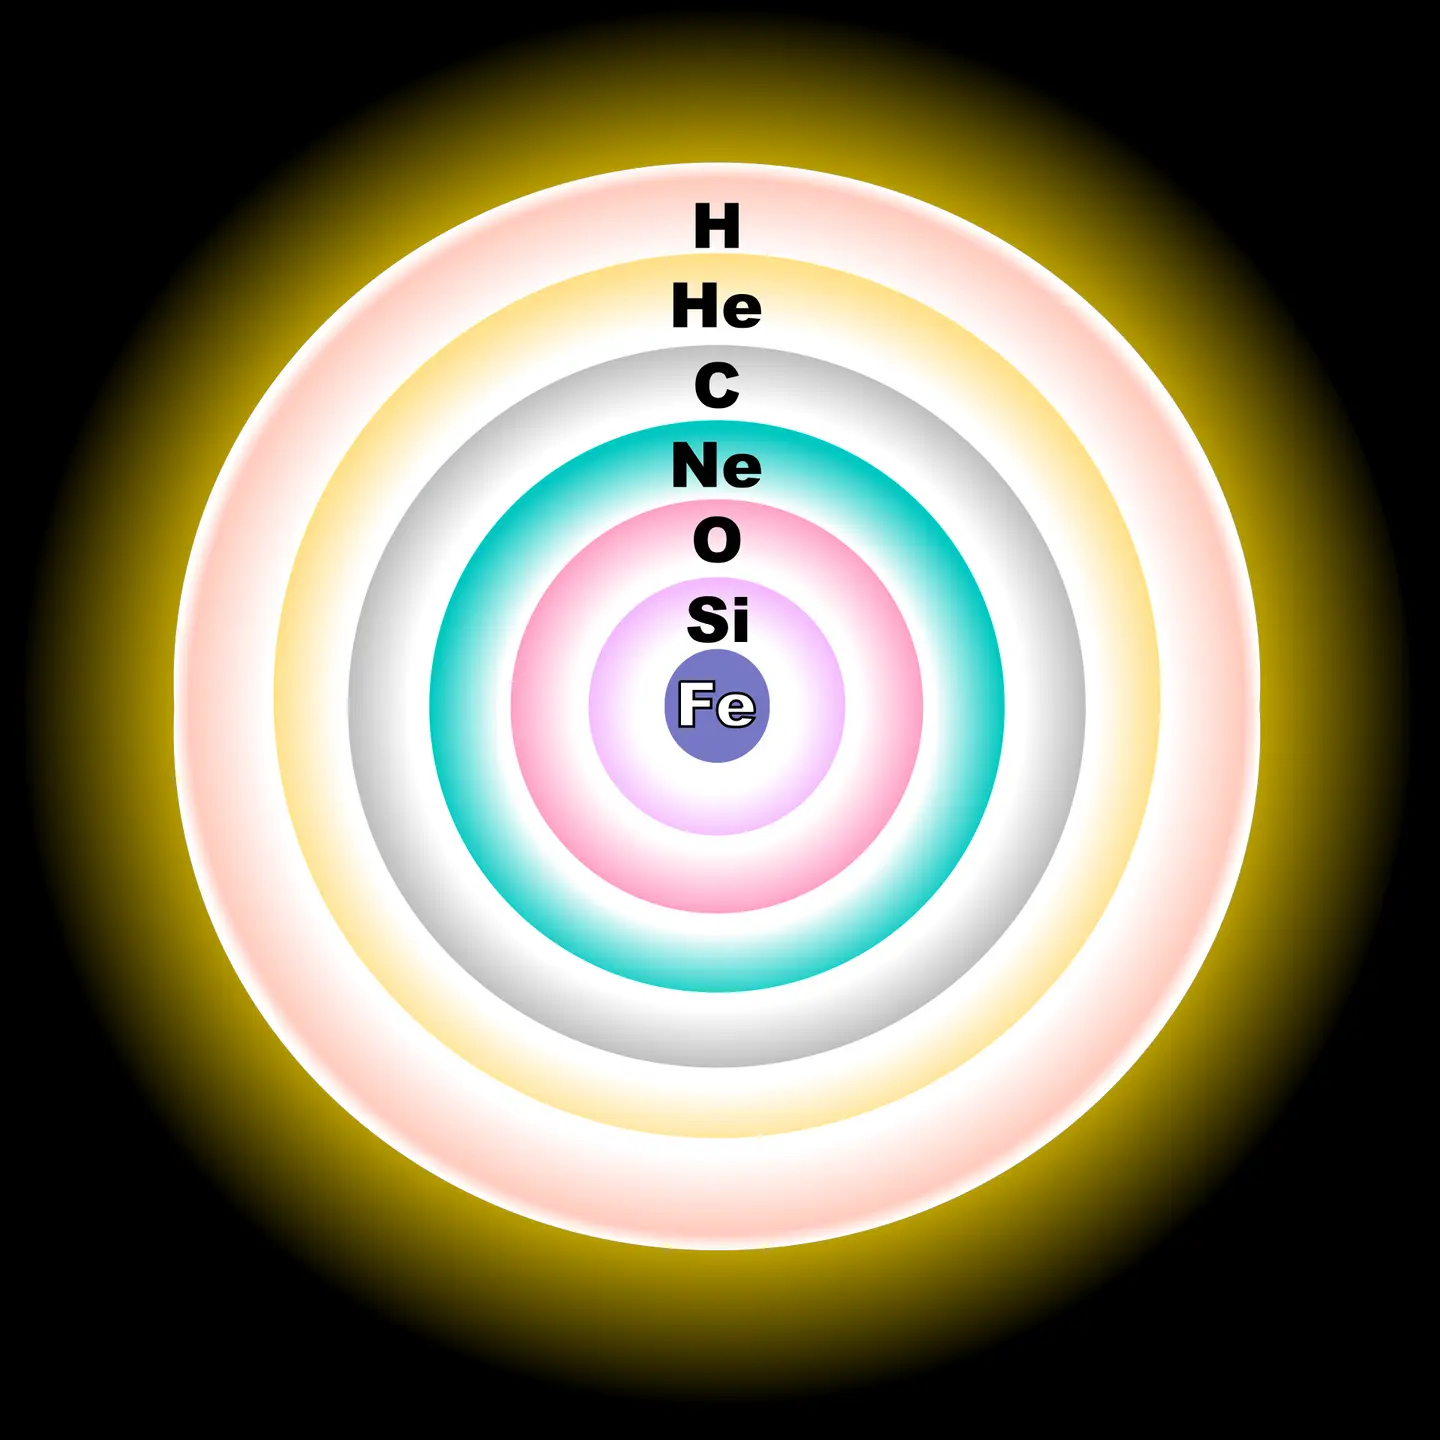
\includegraphics[width=7cm]{figures/figure2_2.JPG}
\captionsetup{justification=raggedright, singlelinecheck=false}
\caption{大质量恒星内部结构示意图。}
\label{大质量恒星内部结构示意图。}
\end{figure}

\subsubsection{能量传输和恒星振荡}
接下来我们研究能量在恒星内部的传输。首先建立能量守恒方程。记单位时间内通过半径为$r$的球面的能量为$L\left(r\right)$,单位物质在单位时间产生的能量(来自核反应和引力势能转换)为$\varepsilon\left(r\right)$,那么半径为$r$,厚度为$\mathrm{d}r$的球壳两侧的能量差为
\begin{equation}
\mathrm{d}L_{r}=L\left(r+\mathrm{d}r\right)-L\left(r\right)=\varepsilon\mathrm{d}M_{r}=4\pi{}r^{2}\rho\varepsilon\mathrm{d}r.
\end{equation}

恒星是稳定的气体球,其内部任意一点必须维持流体静力学平衡,而恒星内部核反应速率$\varepsilon$对温度十分敏感。温度上升势必导致反应速率上升,进而导致压强上升,强过小体元所受的引力,恒星核心区膨胀导致温度下降,形成负反馈,产生$\varepsilon$机制振荡。

能量传输有三种形式:辐射、传导和对流。太阳核心产生的能量主要通过辐射与对流 (convection) 向外传递。习惯上,我们用温度梯度来描述二者的贡献:
\begin{equation}
\frac{\mathrm{d}T}{\mathrm{d}r}=\left.\frac{\mathrm{d}T}{\mathrm{d}r}\right\vert{}_{\text{rad}}+\left.\frac{\mathrm{d}T}{\mathrm{d}r}\right\vert{}_{\text{conv}}.
\end{equation}

首先考虑辐射部分。其实我们已经推导过了,在介绍 Eddington 光度时就考虑过辐射压和引力的平衡,在推导质光关系时将其扩展得到
\begin{equation}
\frac{GM}{r^{2}}=\frac{1}{\rho}\frac{\mathrm{d}P}{\mathrm{d}r}=\frac{1}{c}\kappa\frac{L}{4\pi r^{2}}=\frac{1}{\rho}\frac{4}{3}a_{\text{B}}T^{3}\frac{\mathrm{d}T}{\mathrm{d}r},\tag{\ref{1.4.11}}
\end{equation}
稍作整理并修正下正负号便是所需要的方程
\begin{equation}
\frac{\mathrm{d}T}{\mathrm{d}r}=-\frac{3}{4a_{\text{B}}c}\frac{\kappa\rho}{T^{3}}\frac{L_{r}}{4\pi r^{2}}.
\end{equation}
可见不透明度$\kappa$会影响辐射能传输的效率。不透明度下降,散逸的能量增多,导致核心区温度下降,导致压强下降恒星收缩,密度上升,进而导致不透明度上升,产生$\kappa$机制振荡。

当恒星内部的不透明度或产能率增大时,辐射温度梯度值也随之增大,半径增加一点温度快速下降,说明辐射不再是传递能量的有效方式,恒星依靠对流传递能量。或者当辐射平衡不稳定时,也会产生对流。对流是气体在冷热区域间大规模的循环流动。热气体膨胀上升,冷却后下沉,形成物质流动的循环和能量的传递。对流不仅传递能量,还起到混合物质的作用。

我们可以研究一下绝热条件下的温度梯度。假设恒星内部流体元在上升过程中绝热膨胀,不与周围交换热量,根据
\begin{equation}
P_{\text{g}}=\frac{\rho k_{\text{B}}T}{\mu m_{\mathrm{H}}}
\end{equation}
和
\begin{equation}
P=K\rho^{\gamma}
\end{equation}
可知
\begin{align}
\frac{\mathrm{d}P}{\mathrm{d}r}&=-\frac{P}{\mu}\frac{\mathrm{d}\mu}{\mathrm{d}r}+\frac{P}{\rho}\frac{\mathrm{d}\rho}{\mathrm{d}r}+\frac{P}{T}\frac{\mathrm{d}T}{\mathrm{d}r},\notag\\
\frac{\mathrm{d}P}{\mathrm{d}r}&=\gamma\frac{P}{\rho}\frac{\mathrm{d}\rho}{\mathrm{d}r},\notag\\
\left.\frac{\mathrm{d}T}{\mathrm{d}r}\right\vert{}_{\text{ad}}&=\left(1-\frac{1}{\gamma}\right)\frac{T}{P}\frac{\mathrm{d}P}{\mathrm{d}r}=-\left(1-\frac{1}{\gamma}\right)\frac{\mu m_{\mathrm{H}}}{k_{\text{B}}}\frac{GM_{r}}{r^{2}}.
\end{align}
我们认为$\left\vert{}\dfrac{\mathrm{d}T}{\mathrm{d}r}\right\vert{}_{\text{actual}}<\left\vert{}\dfrac{\mathrm{d}T}{\mathrm{d}r}\right\vert{}_{\text{ad}}$的是辐射区,反之是对流区。

$M>1.5\text{\textendash}2\,M_{\odot}$的恒星,拥有对流核区和辐射包层,核区发生$\mathrm{CNO}$循环核反应,产生能量的内核很小。

$0.8\,M_{\odot}<M<1.5\text{\textendash}2\,M_{\odot}$的恒星,拥有辐射核区和对流包层,核心区发生 pp chain 核反应,能量产生于较大的内核。

$0.1\,M_{\odot}<M<0.8\,M_{\odot}$的主序星,低温,整体对流。

\subsubsection{恒星的物态方程和气体总压强}
恒星内部的总压强主要由两部分组成:气体粒子运动产生的气体压强$P_{\text{g}}$和光子辐射压$P_{\text{rad}}$.不同的物态将会给出不同的压强形式。

对于非简并气体,我们在介绍质光关系的时候就计算过辐射压
\begin{equation}
P_{\text{rad}}=\frac{1}{3}a_{\text{B}}T^{4}.
\end{equation}
而对于气压,我们假设非简并气体状态方程为理想气体状态方程
\begin{equation}
P=nk_{B}T,
\end{equation}
其中$n$是粒子数密度。记气体一共包含$n'$摩尔的分子,那么
\begin{equation}
n=\frac{n'N_{\text{A}}}{V}=\frac{n'N_{\text{A}}}{\dfrac{m}{\rho}}=\frac{\rho}{\dfrac{m}{n'N_{\text{A}}}}=\frac{\rho}{\mu m_{\mathrm{H}}},
\end{equation}
其中$N_{\text{A}}$是阿伏伽德罗常数,$\mu$为平均相对分子质量,$m_{\mathrm{H}}$是质子的实际质量,数值上等于$\dfrac{1}{N_{\text{A}}}$.故非简并理想气体的气压可以写作
\begin{equation}
P_{\text{g}}=\frac{\rho k_{\text{B}}T}{\mu m_{\mathrm{H}}}.
\end{equation}
进一步,我们需要确定恒星中气体的相对分子量。考虑完全电离情形。记$n_{i}$是各元素数密度,$\chi_{i}$是各元素的质量分数,$Z_{i}$是该元素的质子数(电荷数),$A_{i}$是该元素的质量数(即质子和中子数和),那么气压将是电子气体气压和各离子气体气压之和
\begin{equation}
P_{\text{g}}=n_{\text{e}}k_{\text{B}}T+\sum_{i}n_{i}k_{\text{B}}T=\sum_{i}\left(Z_{i}+1\right)n_{i}k_{\text{B}}T=\sum_{i}\left(1+Z_{i}\right)\frac{\rho\chi_{i}k_{\text{B}}T}{A_{i}m_{\mathrm{H}}}=\frac{\rho k_{\text{B}}T}{\mu m_{\mathrm{H}}}.
\end{equation}
因此相对分子量为
\begin{equation}
\frac{1}{\mu}=\sum_{i}\left(1+Z_{i}\right)\frac{\chi_{i}}{A_{i}}.
\end{equation}
如果不考虑电子气体的贡献,即只有一大堆离子,那么
\begin{equation}
\frac{1}{\mu}=\sum_{i}\frac{\chi_{i}}{A_{i}}.
\end{equation}
习惯上,我们记$\mathrm{H},\mathrm{He}$和金属元素的质量百分比$\chi_{i}$分别为$X,Y,Z$,且认为金属元素质子数与中子数相当,即$\dfrac{Z_{i}}{A_{i}}=\dfrac{1}{2}$,那么对于考虑电子气体的情况,
\begin{equation}
P_{\text{g}}=\rho k_{\text{B}}T\frac{2X+\dfrac{3}{4}Y+\dfrac{1}{2}Z}{m_{\mathrm{H}}}.
\end{equation}
若不考虑,
\begin{equation}
P_{\text{g}}=\rho k_{\text{B}}T\frac{X+\dfrac{1}{4}Y}{m_{\mathrm{H}}}.
\end{equation}
同时我们还能给出电子气体的相对分子质量来表征其贡献
\begin{equation}
\mu_{e}^{-1}=\sum_{i}\frac{Z_{i}\chi_{i}}{A_{i}}\approx X+\frac{1}{2}(1-X)=\frac{1+X}{2}.
\end{equation}

当引力越来越强时,即使密度不断提高,理想气体所提供的气压也不足以抗衡引力,此时电子简并压逐渐发挥主导作用。根据泡利不相容原理,电子不可能占据两个相同的能态,宏观上呈现出一定的抗压缩性。对于非相对论性 ($v_{e}\ll c$) 电子,$P_{e}\propto\rho^{\frac{5}{3}}$,对于相对论性电子,$P_{e}\propto\rho^{\frac{4}{3}}$.

\subsubsection{多方球模型}
结合边界条件:$r=0$时,$M\left(r\right)=0,L=0$; $r=R$时,$M\left(r\right)=M,T\left(r\right)=0,P\left(R\right)=0$.

恒星的多方球模型 (Polytropic Model).首先我们假设恒星是球对称结构,各物理量只与半径有关。其次,主序星处于完全流体静力学平衡,压强(来自气压和辐射压)梯度与引力平衡,得到
\begin{align}
\frac{GM_{r}\rho\mathrm{d}A\mathrm{d}r}{r^{2}}&=\left(P\left(r\right)-P\left(r+\mathrm{d}r\right)\right)\mathrm{d}A=-\mathrm{d}P\left(r\right)\mathrm{d}A,\\
\frac{\mathrm{d}P}{\mathrm{d}r}&=-\frac{GM_{r}\rho}{r^{2}}.\\
\frac{\mathrm{d}}{\mathrm{d}r}\left(\frac{r^{2}}{\rho}\frac{\mathrm{d}P}{\mathrm{d}r}\right)&=-G\frac{\mathrm{d}M_{r}}{\mathrm{d}r}=-G\left(4\pi r^{2}\rho\right).\\
\frac{1}{r^{2}}\frac{\mathrm{d}}{\mathrm{d}r}\left(\frac{r^{2}}{\rho}\frac{\mathrm{d}P}{\mathrm{d}r}\right)&=-4\pi{}G\rho.
\end{align}
进一步假设恒星内部气体热量传输符合多方过程,即满足
\begin{equation}
P=K\rho^{1+\frac{1}{n}}=K\rho^{\gamma},
\end{equation}
如此一来压力引力平衡方程可以改写为
\begin{equation}
\left(\frac{n+1}{n}\right)\frac{K}{r^{2}}\frac{\mathrm{d}}{\mathrm{d}r}\left(r^{2}\rho^{\frac{1}{n}-1}\frac{\mathrm{d}\rho}{\mathrm{d}r}\right)=-4\pi G\rho.\label{1.4.7}
\end{equation}
接着作代换
\begin{align}
\rho\left(r\right)&=\rho_{c}\left[\theta_{n}\left(r\right)\right]^{n},\\
r&=a_{n}\xi\left(r\right),\\
a_{n}&=\left[\frac{\left(n+1\right)K}{4\pi G}\rho_{c}^{\frac{1}{n}-1}\right]^{\frac{1}{2}},
\end{align}
其中$\rho_{c}$代表恒星中心的密度,如此一来 (\ref{1.4.7}) 式可以改写为 Lane-Emden 方程的形式:
\begin{equation}
\frac{1}{\xi^{2}}\frac{\mathrm{d}}{\mathrm{d}\xi}\left(\xi^{2}\frac{\mathrm{d}\theta_{n}}{\mathrm{d}\xi}\right)=-\theta_{n}^{n}.
\end{equation}
上式仅在$n=0,1,5$时有解析解:
\begin{align}
\theta_{0}&=1-\frac{\xi^{2}}{6},\\
\theta_{1}&=\frac{\sin\xi}{\xi},\\
\theta_{5}&=\left[1+\frac{\xi^{2}}{3}\right]^{-\frac{1}{2}}.
\end{align}
其结果表明恒星从表面到中心密度、温度、压强等物理量是单调上升的。

\subsubsection{观测检验}
太阳对流区内的扰动在太阳内部产生各种形式的波动(日震波),表现为在太阳表面气体的起伏振荡(特征速度为几厘米/秒,周期约 5 分钟)和亮度变化。这种振荡可以通过太阳表面谱线的多普勒位移来测定。

由于振动频率可以精确测定,且频率依赖于恒星内部结构,恒星内部不同区域振荡模式不同,我们可以利用太阳的振荡现象研究太阳的内部结构。

中微子是一种不带电、质量极小的亚原子粒子,几乎不与任何物质相互作用。

太阳内部核聚变释放能量的$5\%$被中微子携带向外传输。

目前接收到的太阳的辐射实际上产生于$10^{5}\sim10^{7}$年前的太阳内部,而中微子几乎产生于现在。

中微子会和四氯乙烯相互作用,生成半衰期$35$天的$\rm Ar$
\begin{equation}
\rm ^{37}Cl+\nu_e\to{}^{37}Ar+e^-\\
\end{equation}

也可以用纯水进行探测,中微子撞击电子将能量传递给电子后高速电子会产生切伦科夫辐射。

中微子在传播过程中发生了转换。太阳内部核反应只产生$e$中微子,途中会产生$\mu$中微子和$\tau$中微子。表现为探测器白天黑夜得到的结果不一致(夜晚中微子穿过地球走的距离更长)

2001 年加拿大萨德伯里探测器测量到三种中微子,其中 35\%是电子中微子。

\subsection{恒星的演化}
恒星的一生是与引力斗争的一生。

恒星通过核反应产生能量,维持热平衡和流体静力学平衡,同时改变了自身的组成与结构。

Russell-Vogt 原理:如果恒星处于流体静力学平衡和热平衡,而且它的能量来自内部的核反应,它们的结构和演化就完全唯一地由初始质量和化学丰度决定。

恒星演化时标

核时标:恒星核心区(约占总质量的$10\%$)核燃料消耗殆尽所需的时间
\begin{equation}
t_{n}=\frac{E}{L}=\frac{\eta\Delta{}Mc^{2}}{L}\approx0.7\%\times\frac{0.1\,M_{\odot}c^{2}}{L}\approx10^{10}\,\mathrm{yr}\frac{M}{M_{\odot}}\left(\frac{L}{L_{\odot}}\right)^{-1}.
\end{equation}

热时标:恒星辐射完自身内能所需的时间,或者光子从恒星内部到达表面的时间(根据位力定理,内能是引力能的$\dfrac{1}{2}$)
\begin{equation}
t_{\text{the}}=0.5\frac{GM^{2}}{RL}\approx2\times10^{7}\,\mathrm{yr}\left(\frac{M}{M_{\odot}}\right)^{2}\left(\frac{R}{R_{\odot}}\right)^{-1}\left(\frac{L}{L_{\odot}}\right)^{-1}.
\end{equation}

动力学时标:如果恒星内部压力突然消失,引力作用下恒星坍缩的时间
\begin{equation}
t_{\text{dyn}}=\frac{R}{V}\approx\sqrt\frac{R^{3}}{GM}\approx27\,\mathrm{min}\left(\frac{R}{R_{\odot}}\right)^{\frac{3}{2}}\left(\frac{M}{M_{\odot}}\right)^{-\frac{1}{2}}.
\end{equation}



不同质量恒星演化主要区别:

演化过程不同:大质量恒星的内部碳可以点燃,形成更重的元素。

演化时标不同:大质量恒星的内部温度更高;主序星等寿命更短。

演化产物不同:大质量恒星通过超新星爆发,形成中子星或黑洞。

$M_{\odot}<8\,M_{\odot}$的主序星燃烧到最后会剩下一个高温简并 CO 核。恒星的引力要与压力平衡,压力可以来自简并压和普通的气压与辐射压。后两者和温度密度有关,因此会有负反馈调节机制。而前者并没有,因此对于一个 CO 核而言,如果一直添加物质,温度密度一直升高,简并压始终不变,因此温度密度会剧烈上升,直到超过钱德拉塞卡极限(主序质量大于$8\,M_{\odot}$,演化晚期质量大于$1.44\,M_{\odot}$),发生剧烈的热核反应,爆轰,整个星体彻底瓦解,什么也不剩下。

在密近双星(一颗子星影响另一颗子星演化的双星系统)中,双星系统中的白矮星吸积伴星物质,还未超过钱德拉塞卡极限时为新星。一旦超过钱德拉塞卡极限,就会变成\uppercase\expandafter{\romannumeral 1}a 型超新星。因为此刻 CO 核质量都差不多,因此峰值绝对星等大约都是$-19.5$等。

\uppercase\expandafter{\romannumeral 1}型超新星都是双星吸积爆发。\uppercase\expandafter{\romannumeral 1}a 型只有碳氧核,因此没有氢氦,有硅吸收线。\uppercase\expandafter{\romannumeral 1}b 和\uppercase\expandafter{\romannumeral 1}c 是大质量恒星外包层被剥离后的核,其中\uppercase\expandafter{\romannumeral 1}b 没有氢层有氦层,后者氢氦层都被剥离,因此\uppercase\expandafter{\romannumeral 1}b 型有弱氢、强氦吸收线。\uppercase\expandafter{\romannumeral 1}c 型没有氢氦吸收线,有弱硅吸收线。因为\uppercase\expandafter{\romannumeral 1}型超新星爆轰后什么也不会剩下,重金属元素会返还到星际介质中。

一个主序质量大于$8\,M_{\odot}$,演化晚期质量大于$1.44\,M_{\odot}$的星体,最后会发生电子俘获反应,让中微子带走大部分能量,核坍缩到中子简并,包层物质下落,引力能转化成动能产生激波反弹,壳层抛射$\alpha$元素(恒星元素合成主要是氦原子和其他原子碰撞,原子序数$+2+2$地增加),有核心和周围行星状星云残留。因此由大质量恒星直接演化而来的\uppercase\expandafter{\romannumeral 2}型超新星有氢吸收线,重金属也被锁在核心或者黑洞中。

宇宙早期,恒星形成剧烈且质量较大,金属丰度低,此时产生的超新星多是\uppercase\expandafter{\romannumeral 2}型超新星,$\alpha$元素增丰剧烈。就算有小质量恒星,\uppercase\expandafter{\romannumeral 1}型白矮星形成年龄$>40\,\mathrm{Myr}$,也要等到晚期。

等到薄盘形成之时,恒星形成率已显著降低,因此$\alpha$元素增丰显著放缓,而铁族元素由于\uppercase\expandafter{\romannumeral 1}a 超新星的贡献保持相对较快的增丰。

O、B 型恒星表面温度高能产生大量紫外 ($\lambda<912\,\si{\angstrom}$) 光子电离氢,产生$\mathrm{H\uppercase\expandafter{\romannumeral 2}}$区。如斯特龙根球就是年轻 O、B 型恒星周围存在的电离氢区。光致电离产生的大量自由电子之间相互频繁碰撞,建立电子气的平衡态速度分布。

我们相信行星是从小尘埃一路碰撞聚合长成大行星的,一路碰下去能长很大的就比较少;而恒星是从一团很大的气体云坍缩的,坍缩成小团块的概率比较低;褐矮星就卡中间位置了。第四区域请见主序关系。

\subsection{白矮星}

\subsection{中子星}

\subsection{黑洞}


\subsection{行星}
假设行星是黑体,能量全部来自太阳,得到
\begin{equation}
\frac{L_{\odot}}{4\pi R^{2}_{\odot\to\text{planet}}}\pi R_{\text{planet}}^{2}\times\left(1-a\right)=4\pi R_{\text{planet}}^{2}\sigma_{\text{SB}}T_{\text{planet}}^{4}.
\end{equation}
可借此估计行星温度,其中$a$是反照率。

\printbibliography
\end{document}